\documentclass[../TDO4.tex]{subfiles}%

\begin{document}
\section[s]"2"{L'œil hypermétrope et sa correction}

\enonce{%
	Dans cet exercice, on étudie un œil assimilé à une lentille mince convergente
	$\Lc$, dont le centre optique $S$ se trouve à une distance constante $d =
		\SI{17}{mm}$ de la rétine. Cet œil est hypermétrope et donne d'un objet à
	l'infini une image située \SI{1.5}{mm} derrière la rétine lorsqu'il est au repos.
}%

\ifcorrige{%
	\begin{center}
		\begin{tcn}[sidebyside](data){Données}
			\begin{itemize}
				\item Œil = lentille $(\Lc, \rm S)$ ;
				\item $\obarr{SE} = \SI{17}{mm}$ ;
				\item $\obarr{SA} = -\infty \Rightarrow \obarr{SA'} = \obar{\rm
						      SE} + \SI{1.5}{mm}$
			\end{itemize}
			\tcblower
			\begin{center}
				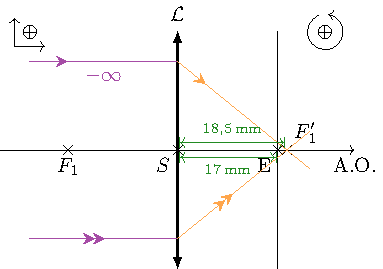
\includegraphics[scale=1]{oeil_hyper-data.pdf}
			\end{center}
		\end{tcn}
	\end{center}
}%

\QR{%
	Déterminer la distance focale de cet œil au repos. On la considèrera
	constante dans la suite du problème, l'œil n'accommodant pas.
}{%
	~
	\begin{tcbraster}[raster columns=5, raster equal height=rows]
		\begin{tcn}(ques){Résultat}
			\[\obarr{SF'}\]
		\end{tcn}
		\begin{tcn}[raster multicolumn=2](tool)""{Outil}
			On trouve le point focal image d'un système en étudiant l'image d'un
			objet à l'infini.
		\end{tcn}
		\begin{tcn}[raster multicolumn=2](appl)'r'{Application}
			Ici, la lecture de l'énoncé donne directement la réponse~: le
			point focal image et \SI{1.5}{mm} derrière la rétine. On a donc
			\[\obarr{SF'} = \SI{18.5}{mm}\]
		\end{tcn}
	\end{tcbraster}
}%

\QR{%
	L'œil est-il trop ou pas assez convergent ? Corrige-t-on ce défaut en
	ajoutant des verres de lunettes convergents ou divergents ?
}{%
	L'œil n'est pas assez convergent, il faudrait que les rayons se
	croisent plus tôt sur l'axe optique pour que l'image se forme sur la
	rétine. Il faut donc corriger avec des lentilles correctrices
	convergentes.


}%

\begin{blocQR}
	\item %
	\enonce{%
		L'œil est corrigé par un verre de lunettes, assimilé à une lentille
		mince de centre optique $O$ et
		placé à une distance $d = \SI{12}{mm}$ du centre optique $S$ de l'œil
		réduit. On souhaite que dans ces conditions, l'œil au repos ait une
		vision nette d'un objet situé à l'infini.
	}%
	\ifcorrige{%
		~
		\begin{center}
			\begin{tcn}[sidebyside](data){Données}
				\begin{itemize}
					\item Verre lunette = $(\Lc_v, \rm O)$ ;
					\item $\obarr{OS} = \SI{12}{mm}$ ;
					\item $\AB \opto{\Lc_v}{\rm O} \ABb \opto{\Lc}{\rm S} \ABp$
				\end{itemize}
				\tcblower
				\begin{center}
					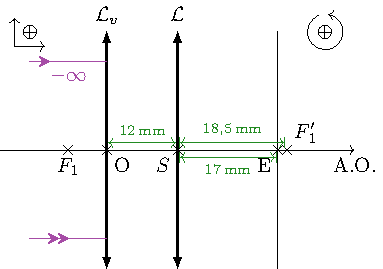
\includegraphics[scale=1]{oeil_hyper-verre.pdf}
				\end{center}
			\end{tcn}
		\end{center}
	}%
	\QR{%
		Rappeler l'endroit où doit se trouver l'image définitive
		donnée par l'œil corrigé.
	}{%
		~
		\begin{center}
			\begin{tcn}(rapp){Rappel}
				L'image doit se former sur l'écran de la lentille,
				autrement dit la rétine~: avec $\AB = -\infty$ on doit
				avoir $\rm A' = E$.
			\end{tcn}
		\end{center}
	}%
	\QR{%
		Quels points caractéristiques du verre et de l'œil doivent
		être confondus afin de corriger la vision de loin ?
	}{%
		~
		\begin{tcbraster}[raster equal height=rows]
			\begin{tcn}(ques){Résultat attendu}
				Utiliser le fonctionnement physique du système pour
				déterminer comment associer la lunette à l'œil.
			\end{tcn}
			\begin{tcn}(appl)'r'{Application}
				\begin{center}
					\begin{tikzpicture}[]
						\node[] (AB) at (0,0) {$\AB$};
						\node[] (A_1B_1) at (2,0) {$\ABb$};
						\node[] (A'B') at (4,0) {$\ABp$};
						\draw[->] (AB) -- (A_1B_1)
						node [midway, above] {$\Lc_v$}
						node [midway, below] {O};
						\draw[->] (A_1B_1) -- (A'B')
						node [midway, above] {$\Lc$}
						node [midway, below] {S};
						\node[below=0.3, Purple!70]
						(AB) at (AB) {$-\infty$};
						\node[below=0.3, brandeisblue]
						(A1B1b) at (A_1B_1) {$A_1 = F'_v$};
						\node[below=0.3, ForestGreen]
						(A1B1bb) at (A1B1b) {$A_1 = R$};
						\node[below=0.3, orange!70]
						(A'B'b) at (A'B') {$A' = E$};
						\draw[->, Purple!70]
						(AB) to[bend right] (A1B1b.west);
						\draw[->, orange!70]
						(A'B'b) to[bend left] (A1B1bb.east);
					\end{tikzpicture}
				\end{center}
				On a donc $\rm A_1 = F'_v = R$.
			\end{tcn}
		\end{tcbraster}
		\begin{tcn}(impo){Important !}
			Attention, \textbf{seul} le remotum de l'œil emmétrope
			est à l'infini. Vérifiez bien vos définitions.
		\end{tcn}
	}%

	\QR{%
		Déterminer la distance focale puis la vergence du verre
		correcteur.
	}{%
		~
		\begin{tcbraster}[raster columns=2, raster equal height=rows]
			\begin{tcn}(ques){Résultats attendus}

				On cherche $\obarr{OF'_v}$ sachant que $\rm F'_v = R$~:
				l'idée est donc de trouver R de l'œil connaissant sa
				distance focale et la distance œil-écran.

			\end{tcn}
			\begin{tcn}(tool)'r'{Outil}

				On va donc utiliser la formule de conjugaison d'une
				lentille mince~:

				\[ \frac{1}{\OFp} = \frac{1}{\OAp} - \frac{1}{\OA}\]
			\end{tcn}
		\end{tcbraster}
		\begin{center}
			\begin{tcn}(appl){Application}
				Avec les données de l'exercice, on a

				\[
					\frac{1}{\obarr{SF'}} =
					\frac{1}{\obarr{SE}} -
					\frac{1}{\obarr{SR}}
				\]
				Soit
				\begin{equation*}
					\boxed{
						\obarr{SR} =
						\frac{
							\obarr{SE}\obarr{SF'}}{
							\obarr{SF'}-\obarr{SE}}
					}
					\quad \text{avec}\quad
					\left\{
					\begin{array}{rcl}
						\obarr{SE}  & = & \SI{17}{mm}   \\
						\obarr{SF'} & = & \SI{18.5}{mm}
					\end{array}
					\right.
				\end{equation*}
				Et
				\[
					\boxed{\obarr{SR} = \SI{21}{cm}}
				\]
				Avec la composition des distances et comme $\rm F'_v = R$,
				on a finalement
				\[
					\boxed{
						\obarr{OF'_v} =
						\obarr{OS} + \obarr{SR} =
						\num{1.2}+\num{20.9} = \SI{22}{cm}}
				\]
				Soit \fbox{$V_{\rm verre} = \SI{+4.5}{\de}$}
			\end{tcn}
		\end{center}
	}%
	\QR{%
		Faire un schéma de principe expliquant la correction de l'œil
		par les lunettes.
	}{%
		On a donc
		\begin{center}
			\hspace*{-2cm}
			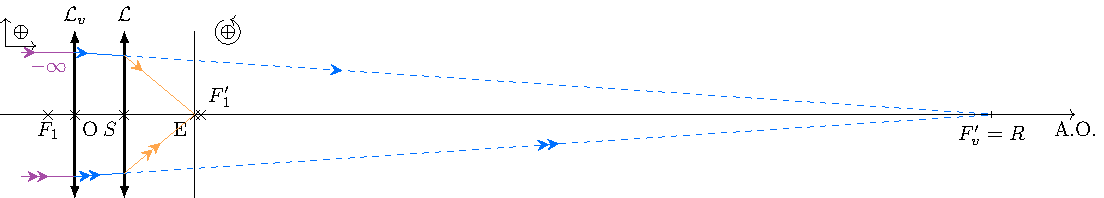
\includegraphics{oeil_hyper-fin}
		\end{center}
	}%
\end{blocQR}

\end{document}
